% begin module tangent-def
\begin{frame}
\begin{columns}[c]
\column{.4\textwidth}
\  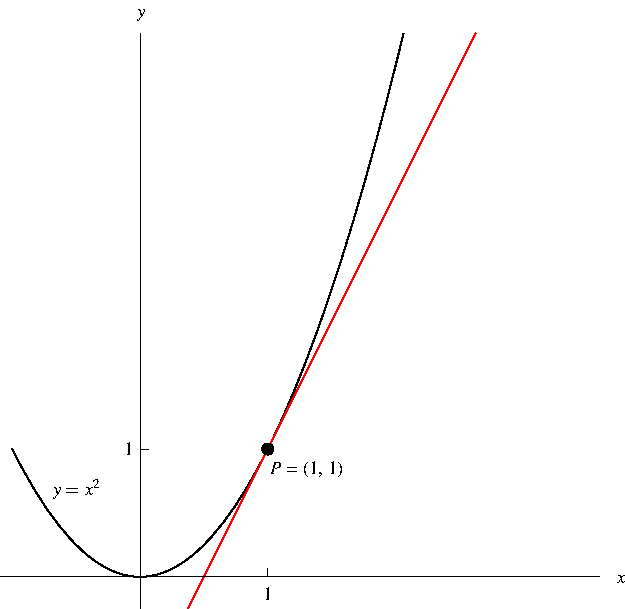
\includegraphics[height=5cm]{limits/pictures/02-01-secanta.pdf}%
\column{.6\textwidth}
We say that the slope of the tangent is the limit of the slope of the secants (limit will be defined later).  We write:
\[
\lim_{Q\rightarrow P} m_{PQ} = m, \qquad \lim_{x\rightarrow 1}\frac{x^2 - 1}{x - 1} = 2 .
\]
\uncover<2->{%
If the slope is indeed $2$, then the equation of the tangent is
\[
y - 1 = 2(x - 1), \qquad \text{ or }\qquad y = 2x - 1.
\]
}
\end{columns}
\end{frame}
% end module tangent-def
